\subsection{Dämpfungsmodellierung}

\begin{frame}
\frametitle{Dämpfungsmodellierung}
        \textbf{\underline{Motivation:}} \\
        Bei geschwindigkeitsproportionaler Dämpfung steigt die pro Zyklus dissipierte Energie
        mit der Frequenz an. In Experimenten tritt diese Frequenzabhängigkeit nicht (ausgeprägt) auf.
\end{frame}

\begin{frame}
        \begin{columns}
                \begin{column}[t]{.5 \linewidth}
                        Something
                \end{column}

                \begin{column}[t]{.5 \linewidth}
                        Federkraft: \\
                        $F_F = k u = k \hat{u} \cos(\overbrace{\omega t - \psi_u}^\varphi)$ \\
                        Dämpferkraft: 
                        $F_D = c \dot{u} = -c \hat{u} \sin(\overbrace{\omega t - \psi_u}^\varphi)$ \\
                \end{column}
        \end{columns}
\end{frame}

\begin{frame}
        Federarbeit pro Zyklus: \\
        $W_F = \int_{+u}^{-\hat{u}} -F_F \ du + \int_{-\hat{u}}^{+\hat{u}} -F_F \ du 
        = \int_{+\hat{u}}^{-\hat{u}} -ku \ du + \int_{-\hat{u}}^{+\hat{u}} -ku \ du = 0$ \\
        Dämpferarbeit (dissipierte Energie) pro Zyklus: \\
        $W_D = \int_{\hat{u}}^{-\hat{u}} -F_D \ du + \int_{\hat{u}}^{-\hat{u}} -F_D \ du$ \\
        \begin{columns}
                \begin{column}[t]{.7 \textwidth}
                        \begin{align*}
                                &= \int_{0}^{\pi} -c \omega \hat{u} \sin^{2}(\varphi) d\varphi
                                + \int_{\pi}^{2\pi} -c \omega \hat{u} \sin^{2}(\varphi) d\varphi \\
                                &= -c \omega \hat{u}^2 |0.5 \varphi| \\
                        \end{align*}
                \end{column}
                \begin{column}[t]{.3 \textwidth}
                        \begin{align*}
                                F_D &= -c\hat{u} \omega \sin(\varphi)\\
                                du &= -\hat{u} \sin(\varphi)\\        
                        \end{align*}       
                \end{column}
        \end{columns}        
\end{frame}

\begin{frame}
        \begin{align*}
                W_D = -c \omega \pi \hat{u}^2 \quad \rightarrow \quad
                \text{Dämpfungskapazität }\psi = \frac{W_D}{\underbrace{0.5 k \hat{u}^2}}\\
        \end{align*}
        Ansatz: $F_D = -k_c \hat{u} \sin(\omega t - \psi_u)$ \\
        \fbox{Das funktioniert nur bei harmonischer Bewegung im eingeschwungenen Zustand} \\
\end{frame}

\begin{frame}
\frametitle{Hysteretische Dämpfung}
        \begin{itemize}
                \item Kraft-Verschiebungsverlauf von Feder und Dämpfer (viskos, hysteretisch) bei harmonischer Bewegung
                \item Leistungsbilanz des Einmassenschwingers im eingeschwungenen Zustand
        \end{itemize}
        \vfill

        \hfill siehe \textsl{V4a.pdf} (handschriftlich)
\end{frame}

%\subsubsection{Komplexe Rechnung}

\begin{frame}
\frametitle{Erinnerungen an Komplexe Zahlen}
\begin{columns}
        \begin{column}[t]{.3\linewidth}
        \begin{tikzpicture}[scale=1.5]
\clip (-1.1, -0.8) rectangle (2,1.5);
\coordinate (Null) at (0,0);
\draw[->] (-1.1, 0) -- (1.25, 0) node[right] {\color{red}Re};
\draw[->] (0, -1.1) -- (0, 1.25, 0) node[above] {\color{green}Im};
\draw[name path=Kreis] (0, 0) circle [radius=1];
\path[name path=Strahl] (0, 0) -- (30:1);
\path[name path=kStrahl] (0, 0) -- (-30:1);
\draw[name intersections={of=Kreis and Strahl, by=Zahl}][blue,semithick] (0,0) -- node[above] {$r$} (Zahl);
\fill[blue] (Zahl) circle[radius=0.03];
\draw (Zahl) node[anchor=south west] {$z$};
\draw[blue] (0.45, 0.1) node {$\varphi$};
\draw[blue,->] (0.6, 0) arc [start angle=0, end angle=30, radius=0.6]; 
\draw[red, semithick] (Null) -- node[below, fill=white] {$a$} (Null -| Zahl);
\draw[green, semithick] (Zahl) -- node[right, fill=white] {$b$} (Zahl|- Null);
\draw[name intersections={of=Kreis and kStrahl, by=kZahl}][blue, dashed] (0,0) -- (kZahl);
\draw (kZahl) node[anchor=north west] {$z^*$};
\fill[blue] (kZahl) circle[radius=0.03];
\end{tikzpicture}

                \begin{align*}
                        z&={\color{red}a}+i{\color{green}b}={\color{blue}r}e^{i{\color{blue}\varphi}}\\
                        z^*&={\color{red}a}-i{\color{green}b}={\color{blue}r}e^{-i{\color{blue}\varphi}}\\
                        |z|&=\sqrt{{\color{red}a}^2+{\color{green}b}^2}={\color{blue}r}\\
                        \sphericalangle z &=\arctan\frac{\color{green}b}{\color{red}a}={\color{blue}\varphi}
                \end{align*}
        \end{column}
        \begin{column}[t]{.7\linewidth}
        \vspace{-3cm}
        \begin{align*}
         \mathrm{Re}\{z\}&={\color{red}a}  ={\color{blue}r}\cos{\color{blue}\varphi}\\
         \mathrm{Im}\{z\}&={\color{green}b}={\color{blue}r}\sin{\color{blue}\varphi}
        \end{align*}
        \hspace{2cm} Ausgewählte Formeln
         \begin{align*}
          z+z^*&=2\,\mathrm{Re}\{z\}\\
          z_1z_2&=r_1r_2 e^{i(\varphi_1+\varphi_2)}\\
          (z_1z_2^*)^*&=z_1^*z_2\\
          (z_1 z_2)^*&=z_1^*z_2^*\\
          \frac{1}{a+ib}&=\frac{a}{a^2+b^2}-\frac{ib}{a^2+b^2}
         \end{align*}
        \end{column}
\end{columns}
\end{frame}


\begin{frame}
        \frametitle{Frequenzgang 1/2}
        Komplexe Erweiterung (Re ``sichtbar'', Im ``mitschleppen'')
        \hspace{1cm}
        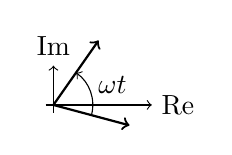
\begin{tikzpicture}[baseline=-1mm]
\draw[->] (-0.1, 0) -- (1.25, 0) node[right] {Re};
\draw[->] (0, -0.1) -- (0, 0.5, 0) node[above] {Im};
\draw[thick,->] (0,0) -- (55: 1); 
\draw[thick,->] (0,0) -- (-15: 1);
\draw[->] (-15:0.5) arc [start angle=-15, end angle=55, radius=0.5];
\draw (0.75, 0.25) node {$\omega t$};
\end{tikzpicture}

        \begin{align*}
        u(t)&= \hat{u}\,e^{i\omega t} &\qquad & \text{mit} \qquad &\hat{u}&=r_u e^{-i\psi_u},\\
        a(t)&=\hat{a}\,e^{i\omega t} &\qquad & \text{mit} \qquad &\hat{a}&=r_a e^{-i\psi_a},\\
        F(t)&= \hat{F}\,e^{i\omega t} &\qquad & \text{mit} \qquad &\hat{F}&=r_F e^{-i\psi_F}.
        \end{align*}
        Standardform des erregten, (viskos) gedämpften Einmassenschwingers
        \begin{equation*}
        \ddot{u}+2\zeta\omega_0 \dot{u}+\omega_0^2 u = \omega_0^2\hat{a}\,e^{i\omega t}.
        \end{equation*}
        Ansatz vom Typ der rechten Seite
        \begin{align*}
        -\omega^2 \hat{u}\,e^{i\omega t} +2i\zeta\omega_0\omega \hat{u}\,e^{i\omega t} +\omega_0^2  \hat{u}\,e^{i\omega t} &= \omega_0^2\hat{a}\,e^{i\omega t},\\
        \left(-\eta^2 + 2i\zeta\eta +1 \right)\hat{u}\,e^{i\omega t}&= \hat{a}\,e^{i\omega t}.
        \end{align*}
\end{frame}

\begin{frame}
\frametitle{Frequenzgang 2/2} 
        \hfill
        $\hat{u}=\underbrace{\frac{1}{1-\eta^2 + 2i\zeta\eta}}_{H(\eta)} \hat{a}$
        \hfill 
        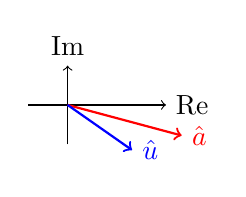
\begin{tikzpicture}[baseline=0mm]
\draw[->] (-0.5, 0) -- (1.25, 0) node[right] {Re};
\draw[->] (0, -0.5) -- (0, 0.5, 0) node[above] {Im};
\draw[thick,red,->] (0,0) -- (-15: 1.5) node[right] {$\hat{a}$};
\draw[thick,blue,->] (0,0) -- (-35: 1) node[right] {$\hat{u}$};
\end{tikzpicture}


        Der Frequenzgang $H(\eta)$ enthält sowohl die Vergrößerungsfunktion $V$ 
        als auch die Phasendifferenz $\psi$
        \only<1>{
        \begin{align*}
        V=|H|&=\left|\frac{1-\eta^2}{(1-\eta^2)^2 + (2\zeta\eta)^2}-
        \frac{2i\eta\zeta}{(1-\eta^2)^2 + (2\zeta\eta)^2}\right| \\
        &= \sqrt{\frac{(1-\eta^2)^2+(2\eta\zeta)^2}{\Bigl((1-\eta^2)^2 + (2\zeta\eta)^2\Bigr)^2}}\\
        &= \sqrt{\frac{1}{(1-\eta^2)^2 + (2\zeta\eta)^2}}
        \end{align*}
        }
        \only<2>{
        \begin{align*}
        \psi=-\,\sphericalangle H &=-\,\sphericalangle \left\{\frac{1-\eta^2}{(1-\eta^2)^2 + (2\zeta\eta)^2}-
        \frac{2i\eta\zeta}{(1-\eta^2)^2 + (2\zeta\eta)^2}\right\}\\
        &=-\arctan\left(\frac{-2\eta\zeta}{1-\eta^2}\right)
        =\arctan\left(\frac{2\eta\zeta}{1-\eta^2}\right)
        \end{align*}

        \vfill
        \alert{\textbf{HA}: Was ändert sich für hysteretische Dämpfung?}
        }
\end{frame}


\begin{frame}
\frametitle{Leistungsbilanz{\normalsize-- Grenzfälle} }
\begin{columns}
        \begin{column}[t]{.5\linewidth}
        \hspace{9mm} Energiespeicher
        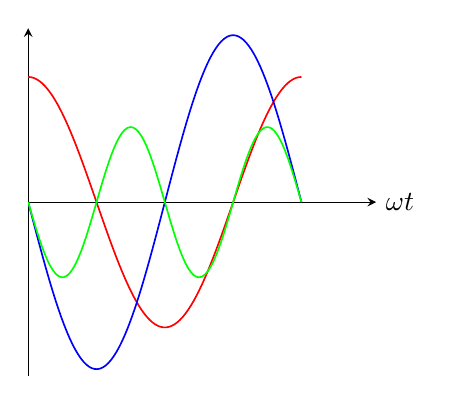
\begin{tikzpicture}
\begin{axis}[
    width=6cm, 
    height=6cm,
    axis x line=center, 
    axis y line=middle, 
    xlabel={$\omega t$},
     x label style={at={(current axis.right of origin)}, right},
    samples=100,
    ymin=-1.25, ymax=1.25,
    xmin=0, xmax=8,
    domain=0.0*pi:2*pi,
    ticks=none
]
\addplot [mark=none, semithick, red] {0.9*cos(deg(x))};
\addplot [mark=none, semithick, blue] {-1.2*sin(deg(x))};
\addplot [mark=none, semithick, green] {-1.2*sin(deg(x))*0.9*cos(deg(x))};
\end{axis}
\end{tikzpicture}  

\bigskip

         Federkraft {\color{red}$F_F$},\\ 
         Geschwindigkeit {\color{blue}$\dot{u}$} und\\
         Momentanleistung {\color{green}$P_F$}
        \end{column}
        \begin{column}[t]{.5\linewidth}
        \hspace{7mm} Energiequelle/-senke
        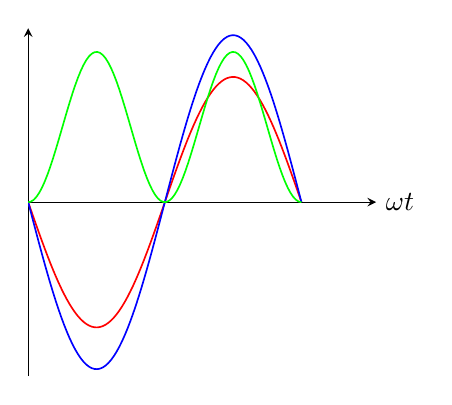
\begin{tikzpicture}
\begin{axis}[
    width=6cm, 
    height=6cm,
    axis x line=center, 
    axis y line=middle, 
    xlabel={$\omega t$},
     x label style={at={(current axis.right of origin)}, right},
    samples=100,
    ymin=-1.25, ymax=1.25,
    xmin=0, xmax=8,
    domain=0.0*pi:2*pi,
    ticks=none
]
\addplot [mark=none, semithick, red] {-0.9*sin(deg(x))};
\addplot [mark=none, semithick, blue] {-1.2*sin(deg(x))};
\addplot [mark=none, semithick, green] {1.2*sin(deg(x))*0.9*sin(deg(x))};
\end{axis}
\end{tikzpicture}      

        \bigskip

         Dämpferkraft {\color{red}$F_D$},\\ 
         Geschwindigkeit {\color{blue}$\dot{u}$} und\\
         Momentanleistung {\color{green}$P_D$}         
\end{column}
\end{columns}
\end{frame}

\begin{frame}
\frametitle{Leistungsbilanz {\normalsize -- Einmassenschwinger 1/3}}
\begin{columns}
        \begin{column}[t]{.5\linewidth}
        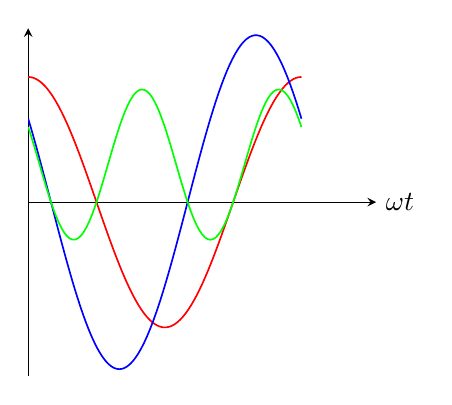
\begin{tikzpicture}
\begin{axis}[
    width=6cm, 
    height=6cm,
    axis x line=center, 
    axis y line=middle, 
    xlabel={$\omega t$},
     x label style={at={(current axis.right of origin)}, right},
    samples=100,
    ymin=-1.25, ymax=1.25,
    xmin=0, xmax=8,
    domain=0.0*pi:2*pi,
    ticks=none
]
\addplot [mark=none, semithick, red] {0.9*cos(deg(x))};
\addplot [mark=none, semithick, blue] {1.2*cos(deg(x)+60)};
\addplot [mark=none, semithick, green] {1.2*cos(deg(x)+60)*0.9*cos(deg(x))};
\end{axis}
\end{tikzpicture} 
     
\bigskip

         Anregende Kraft {\color{red}$F$},\\ 
         Geschwindigkeit {\color{blue}$\dot{u}$} und\\
         Momentanleistung {\color{green}$P$}
        \end{column}
        \begin{column}[t]{.5\linewidth}
        \vspace{-4.5cm}
\begin{align*}
        F&=r_F\,e^{i(\omega t-\psi_a)} \\
        u&=r_u\,e^{i(\omega t-\psi_u)} \\
        &=r_u\,e^{i(\omega t-\psi_a-\psi)} \\
        v&=i\omega r_u\,e^{i(\omega t-\psi_a-\psi)}\\
        &=\omega r_u\, e^{i\frac{\pi}{2}} e^{i(\omega t-\psi_a-\psi)}\\
        & =\omega r_u \,e^{i\left(\omega t+\frac{\pi}{2}-\psi_a-\psi\right)}\\
        r_v&=\omega r_u \\
        \psi_v&=\psi_a+\psi-\frac{\pi}{2}
 \end{align*}
\end{column}
\end{columns}
\end{frame}

\begin{frame}
\frametitle{Leistungsbilanz {\normalsize -- Einmassenschwinger 2/3}}
\begin{align*}
        P&=\mathrm{Re}\left\{F \right\}\mathrm{Re}\left\{v\right\}\\
        &=\frac{1}{2}(F+F^*)\frac{1}{2}(v+v^*)\\
        &=\frac{1}{4}\bigl(Fv+Fv^*+F^*v+F^*v^*\bigr)=\frac{1}{4}\Bigl(Fv+Fv^*+(Fv+Fv^*)^*\Bigr)\\
        &=\frac{1}{2}\mathrm{Re}\left\{Fv+Fv^*\right\}\\
        &=\frac{1}{2}\mathrm{Re}\left\{r_F\,e^{i(\omega t-\psi_a)} r_v\,e^{i(\omega t-\psi_v)}
        +r_F\,e^{i(\omega t-\psi_a)} r_v\,e^{-i(\omega t-\psi_v)} \right\}\\
        &=\mathrm{Re}\left\{\frac{r_F r_v}{2}e^{i(\psi_v-\psi_a)}
        \bigl( e^{i2(\omega t - \psi_v)} + 1  \bigr) \right\}\\
\end{align*}

\end{frame}

\begin{frame}
\frametitle{Leistungsbilanz {\normalsize -- Einmassenschwinger 3/3}}
        \begin{equation*}
                P=\mathrm{Re}\left\{P_S
                \bigl( e^{i2(\omega t - \psi_v)} + 1  \bigr) \right\} 
                \qquad
                \text{mit}
                \qquad
                P_S=\frac{r_F r_v}{2}e^{i(\psi_v-\psi_a)}
        \end{equation*}
Formelsammlung: \quad $\mathrm{Re}\{z_1 z_2\}=\mathrm{Re}\{z_1\}\mathrm{Re}\{z_2\} - \mathrm{Im}\{z_1\}\mathrm{Im}\{z_2\}$
\begin{align*}
   P&=\mathrm{Re}\left\{P_S\right\}\mathrm{Re}\left\{ e^{i2(\omega t - \psi_v)} + 1  \right\}
   -\mathrm{Im}\left\{P_S\right\}\mathrm{Im}\left\{ e^{i2(\omega t - \psi_v)} + 1  \right\}\\
   &=\mathrm{Re}\left\{P_S\right\}\Bigl( \cos(2\omega t - 2\psi_v) + 1 \Bigl)
   -\mathrm{Im}\left\{P_S \right\} \sin(2\omega t- 2\psi_v)
\end{align*}
Damit ist die Momentleistung (Scheinleistung $|P_S|$) dargestellt als Summe eines schwellenden Verlaufs (Wirkleistung $\mathrm{Re}\left\{P_S\right\}$) und eines mittelwertfreien Verlaufs (Blindleistung $\mathrm{Im}\left\{P_S \right\}$). 

\end{frame}

%%%%%%%%%%%%%%%%%%%%%%%%%%%%%%%%%%%%%%%%%%%%%%%%
